% PROTOTYPE of the figure-first rewrite (2026-10-17). Not the manuscript.
% Source of every number: supplement/number-trace-direction2.md (row numbers in % comments);
% Source of the N and C rows cited in % comments: prototype/NEW-TRACE-ROWS.md.
% Figures: figs/ (TikZ sources + one restyled data plot); placeholders drawn by \placeholder.
% Names: design R of earlier drafts is design G here (runs SR, XR are SG, XG); the displacement
% coefficient vector is q, the thickness field h, the sinc matrix S (symbol clashes, referee M11).
% Trim pass (2026-10-17): section numbers 1-9 kept; secondary material moved to Appendices A-G
% after the references (see prototype/TRIM-NOTES.md). Backup: manuscript_proto_voice.tex.bak-trim.
\documentclass[preprint,12pt]{elsarticle}
\usepackage{amsmath,amssymb,bm,booktabs,graphicx,array}
\usepackage{jsvfigs}
\usepackage[section]{placeins}
\usepackage[hidelinks]{hyperref}
\graphicspath{{figs/}}
\journal{Journal of Sound and Vibration}
\biboptions{numbers,sort&compress}
\setlength{\emergencystretch}{3em}
\setlength{\marginparwidth}{18mm}

% ------------------------------------------------------------------ prototype helpers
% Placeholder frame of the planned print size: #1 width, #2 height, #3 inventory id,
% #4 reader question, #5 planned content, #6 data or source.
\newcommand{\placeholder}[6]{%
  \begin{tikzpicture}
    \draw[reference] (0,0) rectangle (#1,-#2);
    \node[anchor=north west, text width=#1-8mm, align=left, inner sep=0pt, outer sep=0pt]
      at (4mm,-3.5mm) {%
      \textbf{PLACEHOLDER (figure not yet drawn) \,|\, inventory #3}\\[3pt]
      \textbf{Reader question:} #4\\[2pt]
      \textbf{Planned content:} #5\\[2pt]
      \textbf{Data / source:} #6};
  \end{tikzpicture}}
% Margin flag for any number that is not in the number trace (none is used at present).
\newcommand{\protonote}[1]{\marginpar{\raggedright\figfontsmall prototype: #1}}
% Include a drawn figure if its PDF exists, else fall back to a placeholder.
% (the 1 mm standalone border is blank, so a 138 mm PDF is centered in the 137 mm text width)
\newcommand{\figorplaceholder}[2]{\IfFileExists{figs/#1.pdf}{\makebox[\linewidth][c]{\includegraphics{#1.pdf}}}{#2}}
% float placement: allow large top floats so figures sit with their text
\renewcommand{\topfraction}{0.9}
\renewcommand{\bottomfraction}{0.6}
\renewcommand{\textfraction}{0.1}
\renewcommand{\floatpagefraction}{0.75}
\setcounter{topnumber}{2}
\setcounter{totalnumber}{3}
% appendix floats: number per appendix (A.1, B.1, ...), with unique hyperref anchors
\makeatletter
\newcommand{\appendixfloats}{%
  \@addtoreset{figure}{section}\@addtoreset{table}{section}%
  \renewcommand{\theHfigure}{app.\Alph{section}.\arabic{figure}}%
  \renewcommand{\theHtable}{app.\Alph{section}.\arabic{table}}%
  \renewcommand{\theHequation}{app.\Alph{section}.\arabic{equation}}%
  \renewcommand{\floatpagefraction}{0.5}}
\makeatother

\begin{document}
\begin{frontmatter}
\title{When is a piston good enough? Limits of radiation simplifications for shell optimization and numerical benchmarks}
\author{Guilherme Henrique da Silva}
\author{Arcanjo Lenzi}
\address{Laborat\'orio de Vibra\c{c}\~oes e Ac\'ustica, Department of Mechanical Engineering, Universidade Federal de Santa Catarina, Florian\'opolis, Brazil}
\begin{abstract}
Shell optimization often computes radiated sound power with the sinc radiation matrix, exact only for a flat surface in a rigid baffle. We ask when such an inaccurate model still produces a good design, judged by its exact radiated power. The test object is a zero-thickness open spherical cap whose faces share one normal velocity; an exact two-sided solution is the reference. For velocity fields frozen at their 100~Hz shapes, the sinc-to-two-sided power ratio exceeds one by orders of magnitude for acoustically small caps, falls to minima of 0.15 to 0.25 near $ka=1.5$--2, and approaches 0.5 for $ka\gtrsim5$ and smooth fields. At 100~Hz ($ka\approx9$) the sinc model predicted its own reductions to within 0.18~dB, yet from one uniform start a sinc-driven descent ended 9.5~dB above the exact-driven one. Over seven combinations of opening and $kR$, the sinc-driven designs were 26 to 50~dB louder than the best exact design at $kR\le3$, with reductions overstated by 16 to 35~dB, but within the exact optimizer's own spread at $kR\ge7$. The low-$kR$ exact designs cancel down to radiation efficiencies of $10^{-8}$ and below; coupled with the fluid, they lost 2 to 15~dB in the scaled medium of the study and 20 to 30~dB with the air density, while the sinc designs stayed 18 to 36~dB louder there, so the exact operator keeps its advantage only with the fluid in the model. The gaps are lower bounds from iteration-limited runs; finite thickness was not examined.
\end{abstract}
\begin{keyword}
Radiated sound power \sep Radiation matrix \sep Rayleigh integral \sep Unbaffled shells \sep Spherical cap \sep Structural-acoustic optimization \sep Benchmarks
\end{keyword}
\end{frontmatter}

% =================================================================== 1
\section{Introduction}
\label{sec:intro}
% Reader question: why does the radiation model matter for a shell design, and what is asked here?
A shell can vibrate with a small amplitude and still radiate a considerable amount of acoustic power. The radiated power depends on the normal velocity of the surface, and also on how the contributions of different points combine in the fluid. A quadratic form in the surface velocity describes both effects: its matrix, the radiation matrix, holds the acoustic interaction between every pair of surface points. Radiation matrices are established tools for sound-power prediction and active control \cite{Borgiotti1990,ElliottJohnson1993,CunefareCurrey1994,LiGibeling2000}, and for objective functions in structural-acoustic design \cite{Constans1998,DuOlhoff2007sound,DuhringJensenSigmund2008}. This paper asks what happens when the matrix of one problem is used for another (Fig.~\ref{fig:problem}).

\begin{figure}[t]
\centering
\includegraphics{fig_cap_problem.pdf}
\caption{The two problems compared in this paper. (a) Flat patch in an infinite rigid baffle, radiating into one half-space; for this configuration the sinc kernel $j_0(k|\bm x-\bm y|)$ gives the exact power. (b) Open spherical cap in free space, the problem solved here. Both faces touch the fluid, the unit normal $\bm n$ points to the outer face, and the pressure difference $\mu=p^+-p^-$ vanishes at the free edge. Schematic; (b) is drawn to scale for $R=10$~m and $\theta_0=30^\circ$, so that $a=5$~m and $ka\approx9.2$ at 100~Hz.}
\label{fig:problem}
\end{figure}

Using the radiation matrix to design a shell raises three difficulties. The most basic one lies in the acoustic model. For a flat surface in an infinite rigid baffle the radiation matrix is known in closed form. Its kernel is $\sin(kr)/(kr)$, where $k$ is the acoustic wavenumber and $r$ is the distance between two surface points; we call it the sinc kernel. The kernel is exact for the configuration of Fig.~\ref{fig:problem}(a). Being real and smooth, and needing no boundary-element solution, it has been applied unchanged to curved shells without a baffle, for example in the thesis on which this paper builds \cite{daSilva2024}. That step changes the physical problem (Fig.~\ref{fig:problem}b): a free open shell has fluid on both faces and a free edge around which the fluid can move, whereas the sinc model gives twice the power of one free-space source layer (Fig.~\ref{fig:factortwo}). For flat plates, the difference between baffled and unbaffled radiation has been studied in detail \cite{Laulagnet1998,Nelisse1998}, and so has the open-back versus closed-back comparison for a rigid oscillating disc in free space \cite{MellowKarkkainen2024}. Approximate power models have been compared with full acoustic solutions for engineering structures \cite{Herrin2006,Fritze2009}, and a plane-projection Rayleigh integral has been compared with analytical sphere solutions \cite{Walther2025}.

\begin{figure}[t]
\centering
\figorplaceholder{fig_factor_two}{\placeholder{137mm}{55mm}{F2}{Why is $P_{\rm sinc}=2P_{\rm mono}$, and why is the open shell neither?}{(a) baffled patch; (b) patch plus mirror image in free space; (c) open shell as a dipole layer.}{Schematic; manuscript Sec.~2.2.}}
\caption{Where the factor two comes from. (a) Flat patch in a rigid baffle; (b) the same patch and its mirror image in free space, which give the same pressure above the plane, so that $P_{\rm sinc}=2P_{\rm mono}$, where $P_{\rm mono}$ is the power of one free-space layer of monopoles with volume velocity $v_n$ per unit area; (c) an open shell with the same normal velocity on both faces, which radiates as a layer of pressure jumps $\mu$ (a dipole layer) and is neither (a) nor (b). In (b) the image coincides with the patch and is drawn apart for clarity. The Green-function note uses the time factor $e^{-i\omega t}$ (Section~\ref{sec:reference}). Schematic, not to scale.}
\label{fig:factortwo}
\end{figure}

A subtler issue concerns the discretization, since the physics does not fix the matrix alone: the matrix also depends on how the shell velocity is carried to the acoustic surface and on how the double surface integral is evaluated. Compressing the matrix to cut its cost adds yet another numerical choice.

The last concern is the behavior of the matrix inside an optimizer, which does not always need the correct power. A model can miss in three ways: it can misstate the absolute level, misjudge the reduction of a design relative to a baseline, or choose poorly among candidate designs. It can fail the first check and still pass the second, as a constant error cancels in a ratio. The third is the one an optimizer depends on.

Thus, we ask: \emph{when does an inaccurate radiation model still produce a good design}, judged by its exact radiated power?

We answer the question for open spherical caps, because for that geometry the two-sided radiation problem can be solved exactly. Figure~\ref{fig:axes} shows what is varied. Every result depends on three independent choices: the physical acoustic model, the discretization of that model, and the use of the operator, including the optimization method. They form separate axes rather than one ladder of models. Held fixed are the shell model, the mesh, the excitation and, when two operators are compared, the normal velocity field.

\begin{figure}[t]
\centering
\includegraphics{fig_model_axes.pdf}
\caption{Three independent choices behind every result. (a) The physical acoustic model changes the boundary-value problem; $2\times$ sinc rescales the sinc model and has the same minimizer, so it is a calibration of the sinc model. (b) Discretization and compression change only how one kernel is evaluated; bold: the spline-consistent matrix, used for the sinc powers unless stated otherwise. (c) The use of the operator decides what depends on it; frozen-field evaluations test operators, optimization runs test designs. Red dashed: surrogate under test; blue: exact reference. Notes at right: magnitudes from Sections~\ref{sec:axes}, \ref{sec:ratio} and~\ref{sec:opt} and \ref{app:sinc}. Schematic.}
\label{fig:axes}
\end{figure}

To that end, we build an exact two-sided radiation reference for open spherical caps, using dual series equations of the kind treated for scattering by open spherical shells \cite{Vinogradov1978,VinogradovPartI2001,VinogradovPartII2002}, solved here by a Galerkin method, thus, avoiding a boundary-element solution for each new velocity field. The factor of two, the low-frequency behavior of unbaffled plates and the dual-series route for open spherical shells are known. The only use we found of the sinc model on unbaffled curved shells is the thesis this paper builds on \cite{daSilva2024}, so the practice under test is documented here by our own earlier work. What this paper adds is threefold: an exact benchmark for open caps, checked against a boundary-element solution and set against the sinc model over frequency, opening and velocity pattern; a reduction of the exact operator to the structural coefficients, which lets an unchanged adjoint optimizer run on the two-sided power; and, with that optimizer, a regime study that locates where sinc-driven optimization stops producing designs close to the best exact ones, followed by a fluid-loading operator from the same solver that tests whether this finding survives coupling with the fluid. All two-sided results rest on one idealization: a surface of zero thickness whose two faces move with the same normal velocity, in unbounded fluid, without a cavity and, except in that fluid-loading check, without fluid loading of the structure.

Sections~\ref{sec:problem} to~\ref{sec:ratio} define the problem and the three errors, test the exact reference and map where the sinc model gives the right power. From Section~\ref{sec:opt} on, the paper turns to designs, at the design point and then over seven combinations of opening and $kR$, in vacuo and with fluid loading, before condensing the outcome into a decision chart with its limits; the appendices after the references hold the verification details, secondary operator tests and benchmark cards.

% =================================================================== 2
\section{Problem statement}
\label{sec:problem}
% Reader question: what is the object, what is computed, and how is an error measured?
\subsection{The shell and its normal velocity}
\label{sec:shell}
The domain of the problem, shown in Fig.~\ref{fig:problem}(b), is an open spherical cap of radius of curvature $R=10$~m and half-angle $\theta_0=30^\circ$. % rows 1-2
Its rim radius is $a=R\sin\theta_0=5$~m, so $ka=kR/2$. At the design frequency of 100~Hz, with sound speed $c_0=343$~m/s and density $\rho_0=1.21$~kg/m$^3$, $kR=18.32$. For a field of element thicknesses $h$, the discrete shell equilibrium at angular frequency $\omega$ is:
\begin{equation}
  \mathbf K_D(h,\omega)\,\mathbf q=\mathbf F,
  \qquad \mathbf K_D=\mathbf K(h)-\omega^2\mathbf M(h)+i\omega\mathbf C(h),
\end{equation}
where $\mathbf K$, $\mathbf M$ and $\mathbf C$ are the stiffness, mass and damping matrices, $\mathbf F$ is the load vector and $\mathbf q$ holds the displacement coefficients. The structural equations use complex amplitudes with the time factor $e^{i\omega t}$, where $t$ is time. The acoustic models need the normal velocity $v_n=i\omega\,\mathbf n\cdot\mathbf u$, where the displacement field $\mathbf u$ on the mid-surface follows from $\mathbf q$ through the spline basis and $\mathbf n$ is the unit normal. % C1-C6
The fields come from quadratic $C^1$ B-spline Kirchhoff--Love elements \cite{HughesCottrellBazilevs2005,Kiendl2009} on a mesh of 40 elements along the meridian and 24 around the axis, loaded by a harmonic force at the apex; Table~\ref{tab:setup} lists the material, damping, load and supports. The rim support fixes the three displacement components and leaves the rotations free. Acoustically, it is assumed transparent: the fluid moves freely around the rim, as the free-edge condition of Section~\ref{sec:twosided} requires. Fluid loading of the structure is neglected except in Section~\ref{sec:fsi}. The specific acoustic impedance of air, $\rho_0c_0=415$~Pa\,s/m, is about 0.17\% of the mass impedance of the uniform shell, $\omega m''=2.5\times10^5$~Pa\,s/m with $m''=393$~kg/m$^2$; this estimate ignores stiffness and radiation reactance. % N28
The velocity fields are test fields for radiation operators; they are not a validated structural benchmark.

\begin{table}[t]
\centering
\caption{Setup of the shell model and of the optimization runs (Sections~\ref{sec:shell} and~\ref{sec:runs}). The same structural model produced the six frozen fields of Section~\ref{sec:ratio}.}
\label{tab:setup}
\small
\begin{tabular}{>{\raggedright\arraybackslash}p{27mm}>{\raggedright\arraybackslash}p{101mm}}
\toprule
Item & Setting \\
\midrule
Geometry & spherical cap, $R=10$~m, $\theta_0=30^\circ$, $a=5$~m; mid-surface only \\
Shell model & Kirchhoff--Love, quadratic $C^1$ B-splines; $40\times24$ elements (meridian $\times$ circumference), periodic around the axis; 3024 displacement coefficients \\
Material & steel: $E=200$~GPa, $\nu=0.3$, density 7850~kg/m$^3$ \\
Damping & stiffness-proportional, $\mathbf C=\beta\mathbf K$ with $\beta=0.1/\omega$ (loss factor 0.1) \\
Load & harmonic force of 1~N along the axis at the apex, shared equally by the control points of the apex row \\
Supports & rim: three displacement components fixed, rotations free; acoustically transparent \\
Design variables & 960 element thicknesses $h_e$, $25\le h_e\le100$~mm; uniform design and cold start $h_e=50$~mm \\
Constraint & mean element thickness at most 50~mm (elements not weighted by area) \\
Objective & radiated power in dB, scaled by its value at the first iteration \\
Optimizer & GCMMA \cite{Svanberg2002}; at most 20 inner and 600 outer iterations \\
Stopping rule & for three consecutive iterations: relative change below $10^{-4}$ between the mean scaled objectives of two successive 10-iteration windows, largest thickness change below $10^{-4}$ of the bound range, and the volume constraint met to $10^{-6}$ \\
Sinc operator & spline-consistent, $4\times4$ Gauss points per element \\
Exact operator & $\mathbf F_x$ ($1730\times3024$): 48 Galerkin functions per azimuthal order $|m|\le20$; velocity at $8\times8$ Gauss points per element; Richardson step from $L=4000$ and 8000; negative eigenvalues set to zero (Section~\ref{sec:runs}) \\
\bottomrule
\end{tabular}
\end{table}
% Table values: NEW-TRACE-ROWS C1-C13; trace rows 1-2, 16, 77, 79-81.

\subsection{The sinc model and the factor two}
\label{sec:sinc}
For the baffled flat patch of Fig.~\ref{fig:factortwo}(a), the Rayleigh integral gives the pressure, and the time-averaged power becomes a symmetric double integral:
\begin{equation}
 P_{\rm sinc}=\alpha\int_\Gamma\int_\Gamma \overline{v_n(\mathbf x)}\,
 j_0(k|\mathbf x-\mathbf y|)\,v_n(\mathbf y)\,dS_y\, dS_x,
 \qquad \alpha=\frac{\rho_0\omega^2}{4\pi c_0},
 \label{eq:power}
\end{equation}
where $\Gamma$ is the vibrating surface and $j_0(s)=\sin(s)/s$. Applied with source points on a curved shell, Eq.~(\ref{eq:power}) defines what we call the sinc model.

The coefficient $\alpha$ hides a factor two, and Fig.~\ref{fig:factortwo} shows its origin. Removing the baffle and adding a mirror image of the patch leaves the pressure above the plane unchanged. One free-space sheet of monopoles, with volume velocity $v_n$ per unit area, radiates $P_{\rm mono}=\tfrac12P_{\rm sinc}$ on any surface, because the imaginary part of the free-space Green function $e^{ikr}/(4\pi r)$ is $\sin(kr)/(4\pi r)$. We checked this on 300 random points of a non-spherical surface, with $P_{\rm mono}$ computed from its far field: the ratio was 2 to twelve digits at four wavenumbers. % row 5; N31
The identity follows from the monopole-element power model \cite{FahnlineKoopmann1996} together with image doubling for a baffle, and we have not found it stated in this form. Its value here is that it pulls two questions apart: the sinc model is twice one free-space source layer, and whether that matches a real shell depends on how many faces radiate.

\subsection{The two-sided open-shell problem}
\label{sec:twosided}
An open shell in free space has fluid on both faces, and both move with the same normal velocity, so only the jump across the surface enters, $\mu=p^+-p^-$. Here $p^+$ is the pressure on the face to which $\mathbf n$ points (the outer, convex face) and $p^-$ that on the inner face. The exterior Helmholtz problem becomes a hypersingular integral equation:
\begin{equation}
 (\mathcal H\mu)(\mathbf x)=i\omega\rho_0\,v_n(\mathbf x)\ \text{on }\Gamma,\qquad \mu=0\ \text{on the free edge},
 \label{eq:hypersingular}
\end{equation}
where $\mathcal H$ is the normal derivative of the double-layer potential, written with the time factor $e^{-i\omega t}$ of the acoustic solver (Section~\ref{sec:reference}). The jump vanishes at the free edge, since the fluid flows around the rim. The radiated power is:
\begin{equation}
 P_{2s}=\tfrac12\operatorname{Re}\int_\Gamma \mu\,\overline{v_n}\,dS .
 \label{eq:p2s}
\end{equation}

\subsection{Three ways to be wrong}
\label{sec:errors}
We measure the error of the sinc model in three ways, one for each use a designer makes of it. The \emph{absolute power error} is the ratio of the two powers for a given normal velocity:
\begin{equation}
 \rho(d)=\frac{P_{\rm sinc}(d)}{P_{2s}(d)},
\end{equation}
where $d$ denotes a design or, more generally, a velocity field; $\rho<1$ means the sinc model under-predicts.

For a reduction, what counts is the level of a design relative to a baseline $d_0$, here the uniform thickness: $\Delta L_M(d)=10\log_{10}[P_M(d)/P_M(d_0)]$ for a model $M$. The \emph{reduction error}, the predicted minus the true change, is:
\begin{equation}
 e_{\rm red}(d)=\Delta L_{\rm sinc}(d)-\Delta L_{2s}(d)=10\log_{10}\frac{\rho(d)}{\rho(d_0)} .
 \label{eq:ered}
\end{equation}
The second form follows from the definitions. A negative $e_{\rm red}$ means that the sinc model overstates the reduction, and a positive one that it understates it. A large absolute error does no harm to a reduction if $\rho$ is the same for the design and the baseline. The identity also explains why $2\times$ sinc is a calibration: a constant factor changes $\rho$ but neither $e_{\rm red}$ nor the minimizer.

A designer who must choose needs a third measure. The \emph{selection error} judges a design $d$ by its exact power against the best design known under the exact model, $d^\ast$:
\begin{equation}
 s(d)=10\log_{10}\frac{P_{2s}(d)}{P_{2s}(d^\ast)} .
 \label{eq:sel}
\end{equation}
If $d^\ast$ comes from a local method that has not converged, the true optimum is at least as quiet, and $s(d)$ is a lower bound on the suboptimality of $d$.

% =================================================================== 3
\section{Three axes of a radiation model}
\label{sec:axes}
% Reader question: which choices change the physics, and which only change the numbers?
\emph{Physical acoustic model} (Fig.~\ref{fig:axes}a). The sinc model, the exact cap solution of Section~\ref{sec:reference} and a two-sided boundary-element solution are different boundary-value problems. Doubling the sinc power is not a fourth one, because by Eq.~(\ref{eq:ered}) it leaves every reduction, ranking and optimum unchanged.

\emph{Discretization and compression} (Fig.~\ref{fig:axes}b). The discrete sinc matrix depends on the velocity trace and on the surface integration. We use the spline-consistent matrix, which takes the field and the normal from the spline basis at every quadrature point; \ref{app:sinc} gives its construction, the two places where another matrix was used, and the effect of compressing the kernel. Going from the element-centroid matrix of the thesis \cite{daSilva2024} to the spline-consistent one changed the power by 1.33\% for design G and by at most 1.99\% over the six cap fields of Section~\ref{sec:ratio}, minor beside the model error of a factor 1.6 to 2.0 at 100~Hz. % rows 32, 103; 1/0.636 and 1/0.494 from row 54
Compression behaves differently: a low-rank kernel with a normwise error of order $10^{-5}$ underestimated the power of a canceling field by 6\%. % rows 35, 71 (details in Appendix A)

\emph{Use and optimization method} (Fig.~\ref{fig:axes}c). Most comparisons hold a normal-velocity field fixed and change only the operator; we call these fields frozen. A frozen-field evaluation, or a sweep of $kR$ with a frozen field, tests the operators. It does not test an optimization, as at another frequency the shell would vibrate differently and an optimizer would move elsewhere. Design questions are left to the optimization runs of Section~\ref{sec:opt}.

% =================================================================== 4
\section{Can the reference be trusted?}
\label{sec:reference}
% Reader question: is the exact two-sided solution correct?
On a sphere the double-layer operator is diagonal in spherical harmonics. With $x=kR$, the coefficients of the radial velocity and of the pressure difference are related by
\begin{equation}
 \rho_0c_0\,v_{\ell m}=\lambda_\ell\,\mu_{\ell m},\qquad \lambda_\ell=x^2j_\ell'(x)\,h_\ell'(x),
 \label{eq:lambda}
\end{equation}
where $j_\ell$ is the spherical Bessel function and $h_\ell=h_\ell^{(1)}$ the spherical Hankel function of the first kind. The acoustic solver uses the time factor $e^{-i\omega t}$, under which $h_\ell^{(1)}$ is outgoing and $\partial p/\partial n=i\omega\rho_0v_n$; the radiated power does not depend on the convention. The coefficient $\lambda_\ell$ is the ratio of velocity to pressure jump, scaled by $\rho_0c_0$, for a double layer on the complete sphere. % C16
A cap requires $\mu$ to vanish on the rest of the sphere, while $v_n$ is prescribed only on the cap. These dual series equations, of the type treated for open spherical shells \cite{Vinogradov1978,VinogradovPartI2001}, are solved here by a Galerkin method. Its basis functions vanish like the square root of the distance to the edge, with 48 functions per azimuthal order $m$ and $|m|\le20$. % row 16
The velocity enters through its projections on the spherical harmonics, computed by Gauss quadrature of the velocity trace. Besides the basis size, the main approximation is the truncation degree $L$ of the operator sum. Richardson extrapolation from $L=4000$ and 8000 changes the power by $1.3$ to $2.0\times10^{-4}$ for five of the six frozen fields and by $6.7\times10^{-4}$ for design B. % rows 12-13; N18

Two independent checks support the solution; \ref{app:verification} gives them in full. As $a/R\to0$ the cap tends to a flat disc in free space, solved separately in the Hankel-transform domain, and the extrapolated cap power agrees with the disc to between $3\times10^{-5}$ and $5.4\times10^{-4}$ at $ka=0.1$, 1, 3 and 10. % row 19
A boundary-element solution given the same velocity traces as the exact solver agrees with it for six frozen cap fields at 100~Hz to 0.1--0.6\% on the finer of two meshes. % row 23
The truncation is also harmless along the optimization paths of Section~\ref{sec:opt}: for all 3121 designs met there, dropping the Richardson step changes the exact power by at most 0.14\%. % N5
The solution does not, however, resolve combinations of designs that cancel to below about $2\times10^{-3}$ of the power of the designs combined, each normalized to unit exact power; where deeper designs appear, in Section~\ref{sec:pilot}, their resolution is stated with them. % row 105

% =================================================================== 5
\section{Where does the sinc model give the right power?}
\label{sec:ratio}
% Reader question: how large is the absolute power error, and on what does it depend?
\subsection{Ratio against frequency for frozen design fields}
We take six cap fields at 100~Hz from earlier optimization runs of ours with the same structural model, bounds and volume constraint, not published separately. They are the response of the uniform-thickness design (U) and the responses of five optimized designs. Design G minimized the radiated power under the sinc model, in the element-centroid form of Section~\ref{sec:axes}, compressed (\ref{app:sinc}). Designs B to E minimized other objectives: a net-volume-velocity measure, the squared sum of the element-center normal velocities (B); the input power (C); the dynamic compliance (D); and a phase-blind sum of squared velocity coefficients (E). % C15
Holding each normal-velocity field fixed, we change only the acoustic wavenumber in both operators (Fig.~\ref{fig:ratiokR}).

\begin{figure}[t]
\centering
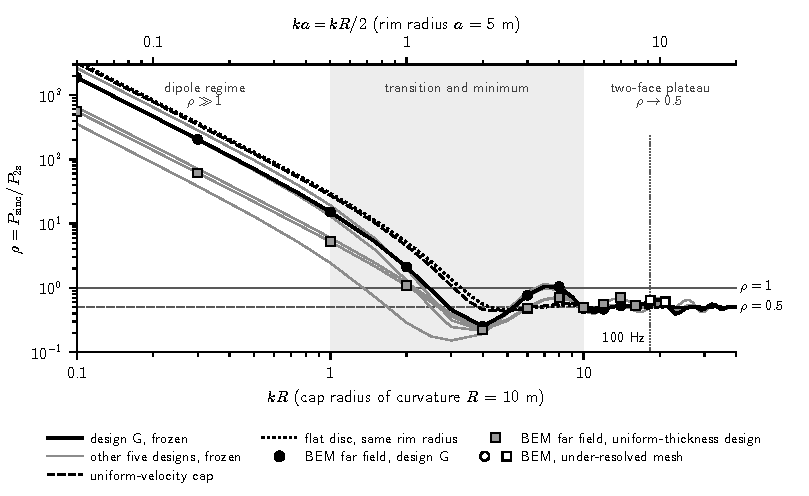
\includegraphics{fig_ratio_kR_proto.pdf}
\caption{Ratio of sinc power to exact two-sided power for six cap fields frozen at their 100~Hz shapes, against $kR$ (bottom) and $ka$ (top). Follow design G (bold) from left to right: from about $2\times10^3$ the ratio falls through one to its minimum near $kR=4$, rises back above one at $kR=7$--8, and then oscillates about 0.5. A uniform-velocity cap (dashed) follows the flat disc of the same rim radius (dotted). Markers: spline-consistent sinc power over the boundary-element far-field power on the coarse mesh, for design G and the uniform-thickness design, open where the mesh has fewer than six elements per wavelength. The regime names and the shaded band are labels, not fitted limits. $R=10$~m, $\theta_0=30^\circ$; the dotted vertical line marks 100~Hz ($kR=18.32$).}
\label{fig:ratiokR}
\end{figure}

Figure~\ref{fig:ratiokR} shows the ratio $\rho$ for $0.1\le kR\le40$, that is $0.05\le ka\le20$. Look first at the left of the figure. When the cap is acoustically small, $\rho$ is far above one: 354 to 2627 at $kR=0.1$, and 2.4 to 19 at $kR=1$. % rows 37-38
The sinc model behaves like a monopole layer there, whereas the two faces of the open shell move together and radiate like a dipole layer, so the two-sided power is 2 to 3 orders of magnitude smaller. Between $kR\approx1$ and 2.5 every ratio falls through one. % row 39
Each field reaches its minimum, 0.15 to 0.25, at $kR=3$ or 4 ($ka=1.5$--2); at $kR=3$ alone the six ratios spread from 0.15 to 0.46, because the curves fall steeply there. % row 40; N23
The minimum is not the end of the transition. Three fields rise back above one at $kR=7$--8, to between 1.05 and 1.15, and a fourth reaches 0.99. % N22
Above $kR\approx10$ ($ka\approx5$) the ratio oscillates about 0.5, within 0.43 to 0.70 up to $kR=27$ and within 0.42 to 0.56 from $kR=28$; at $kR=40$ all six fields lie between 0.495 and 0.504. % row 41; N24

The two reference curves help to read this shape. The flat disc gives the known baffled-versus-unbaffled behavior of flat plates \cite{Laulagnet1998,Nelisse1998} and of rigid discs \cite{MellowKarkkainen2024}, and the uniform-velocity cap follows it closely (3147 against 3327 at $kR=0.1$, 0.47 to 0.53 above $kR=10$). The six design fields follow its shape but not its level: for $kR\le1$ they lie a factor of 1.3 to 11 below it, and near $kR=8$ up to a factor of 2 above it. On one geometry, the velocity pattern alone thus changes the ratio by a factor of up to 7.4 at $kR=0.1$. % N25, N26; row 37
The boundary-element far-field power follows the exact curve (\ref{app:verification}). The ratios of 0.49 to 0.64 at 100~Hz are thus points on an oscillating approach to 0.5, and the sinc model has no constant ratio. % row 43

For the reduction error only the spread of $\rho$ between designs matters, by Eq.~(\ref{eq:ered}). At 100~Hz the six frozen designs have $\rho$ between 0.494 and 0.636, so design G is 17.21~dB quieter than the uniform design under the sinc model and 17.04~dB under the exact model, while design B is 11.18 and 10.08~dB quieter. % rows 54, 55, 59
The reduction errors of the frozen designs follow: $-1.10$~dB for B, $-0.71$, $-0.82$ and $-0.54$~dB for C to E, and $-0.17$~dB for G. The sinc model overstated the reductions of all five, most for B, the design with the lowest ratio. % N1, N2
An optimizer driven by the sinc model can gain from the same effect, since it is credited with more reduction where $\rho$ is low. Here the spread of $\rho$ at 100~Hz is narrow, so that gain is limited to about 1~dB.

\subsection{Beyond $ka$: opening angle, $kR$ and field spectrum}
\label{sec:regime}
One size parameter does not place a case on the map. We evaluated caps with $\theta_0=15^\circ$ to $150^\circ$ under a uniform velocity $v_{\rm c}$ and eight axisymmetric patterns $v_j=\cos\!\left((j+\tfrac12)\pi\theta/\theta_0\right)$, $j=0,\dots,7$, which vanish at the edge and change sign more often as $j$ grows (Fig.~\ref{fig:regime}). For open caps and smooth patterns the ratio stays close to 0.50 above $kR=10$. % row 46
When a small cap carries a rapidly varying pattern, the pattern is subsonic (its structural wavenumber exceeds $k$), so its radiation is expected to come mainly from the edge. The sinc model then over-predicts: the geometric mean over $10\le kR\le40$ reaches 3.3, and single values about 17, at $\theta_0=15^\circ$. % row 44
On the nearly closed cap, $\theta_0=150^\circ$, the ratio oscillates between about 0.05 and 1.8, moving toward the closed sphere with its interior resonances. % row 45
In the cases tested, three quantities were needed to place a case on the map: the acoustic size $kR$, the opening $\theta_0$, and how fast the velocity pattern varies compared with the acoustic wavelength.

\begin{figure}[t]
\centering
\figorplaceholder{fig_regime_map}{\placeholder{137mm}{52mm}{F8}{Where does the sinc model hold across opening angle, frequency and field spectrum?}{Two maps of $\log_2\rho$ over $\theta_0$ (15--150$^\circ$) and $kR$ (0.1--40, log axis): (a) smooth pattern $v_0$, (b) edge-dominated pattern $v_7$; contours at $\rho=1$ and $\rho=0.5$; regions named with leaders (dipole regime; minimum; two-face plateau; edge-dominated subsonic; near-closed resonances). Interpolation between the 49 $kR$ values disclosed.}{novelty/cap\_modes\_ratio.csv (6 openings $\times$ 49 $kR$ $\times$ 9 fields).}}
\caption{Regime map of $\rho=P_{\rm sinc}/P_{2s}$ for open caps of half-angle $\theta_0$. (a) Smooth pattern $v_0$ and (b) edge-dominated pattern $v_7$ against $kR$: red cells mean that the sinc model over-predicts, blue cells that it under-predicts, and the black staircase separates $\rho>1$ from $\rho<1$. Read each row from left to right, from the dipole regime through the minimum to the plateau; the edge-dominated pattern on the $15^\circ$ and $30^\circ$ caps stays mostly above one, and the $120^\circ$ and $150^\circ$ rows alternate, as near a closed sphere. Each cell in (a) and (b) is one computed value, neither averaged nor interpolated; cells span the geometric midpoints between the 49 sampled $kR$, and the color is clipped at $1/8$ and 8 (values at low $kR$ reach $10^5$). (c) Geometric mean of $\rho$ over the 31 sampled $kR$ in $10\le kR\le40$ for the uniform velocity $v_{\rm c}$ and the patterns $v_0$ to $v_7$; at the right, the same mean over the 32 sampled $kR$ (including 100~Hz) for the six frozen design fields at $\theta_0=30^\circ$. The geometric means hide the swing of the $150^\circ$ row. The regime names are descriptive. $kR$ is used rather than $ka=kR\sin\theta_0$, which decreases with the opening for $\theta_0>90^\circ$.}
\label{fig:regime}
\end{figure}

\subsection{Ranking against frequency: an operator test}
\label{sec:ranking}
The spread of $\rho$ between designs also decides whether the two operators put designs in the same order. Over the six frozen fields, the Kendall rank correlation $\tau$ between sinc and exact power equals one at 100~Hz but falls below one at 19 of the 48 frequencies of the sweep, and random combinations of the analytic patterns give a consistent picture on open caps (\ref{app:ranking}). % rows 68-70
The sweep is an operator test: the fields keep their 100~Hz shapes, so it says nothing about the designs an optimizer would reach at another frequency. The lesson it carries is narrower: a matching rank order at one frequency did not guarantee the same order across a band.

\subsection{Is the 0.5 a missing face?}
\label{sec:faces}
The plateau suggests a picture: both faces radiate, and the sinc model counts one. If so, doubling the sinc power should calibrate the level. For the six frozen cap fields at $kR\ge10$, doubling lands within $-16\%$ and $+22\%$ of the exact power (5th to 95th percentile); % row 48
for the analytic patterns at $kR\ge10$ it is within $\pm20\%$ for 92\% of the points at $\theta_0=90^\circ$, but only 34\% at $15^\circ$ and 18\% at $150^\circ$. % row 49
In the dipole regime no constant factor helps, since $\rho$ itself varies sevenfold across the six fields at $kR=0.1$. % row 37
Whether one face accounts for the sinc power depends on how face power is defined, and \ref{app:faces} compares two definitions on one coarse boundary-element mesh. The figure that matters is that at 100~Hz the sinc power lies within $-8\%$ and $+14\%$ of the surface work done by the outer face for the six fields, but far from a far-field half split. % rows 61-62
This is consistent with a one-face picture without establishing it, and away from 100~Hz the match breaks down.

% =================================================================== 6
\section{When does the sinc model still pick a good design?}
\label{sec:opt}
% Reader question: do the reduction and the selection survive the model error?
\subsection{Six optimization runs}
\label{sec:runs}
Frozen fields cannot answer the design question, so we re-optimized the cap thickness at 100~Hz under each operator, with the setup of Table~\ref{tab:setup}. For the continuous problem, the exact operator is a Hermitian positive semidefinite quadratic form in the velocity. It can therefore be written in the structural coefficients as $P_{2s}=\omega^2\|\mathbf F_x\mathbf q\|^2$, where the subscript $x$ marks the exact operator; \ref{app:verification} describes how $\mathbf F_x$ was built from the Galerkin solution, including the clipping of small negative eigenvalues introduced by the extrapolation in $L$. % C12; row 79; N29 (moved to Appendix B)
The factor took 54~s to build and reproduces the exact solution on the six frozen designs to within 0.07\%. % rows 77, 80
The sinc objective has the same form, so the adjoint, optimizer, bounds and stopping rule are shared; both adjoint gradients agree with central differences to $4\times10^{-7}$. % row 78

Each operator was started from the uniform thickness, from design G, and from the end design of the other operator's run from uniform (Table~\ref{tab:opt}). The three starts are not independent, and the uniform thickness is the only cold start shared by both operators. Just one run, the sinc run from design G, met the stopping rule, after 109 iterations. Of the five runs that stopped at the 600-iteration limit, three changed by at most 0.006~dB over their last 100 iterations and run XS by 0.05~dB. % rows 81-84
Run X0, the exact run from the uniform thickness, had not converged: it was still descending by 0.15~dB per 100 iterations, so the local optimum along its path is quieter than the design it returned. % row 84

\begin{table}[t]
\centering
\caption{Cap optimization at 100~Hz under the sinc and exact two-sided operators; all levels in dB. $\Delta L$: power change relative to the uniform design under each model; $\rho$: sinc-to-exact power ratio (0.636 for the uniform design); $e_{\rm red}$: predicted minus true change, Eq.~(\ref{eq:ered}), negative when the sinc model overstates the reduction; $s$: exact-power gap to the best exact design found (X0), Eq.~(\ref{eq:sel}), a lower bound because X0 had not converged. Runs are named by operator (S, sinc; X, exact) and start (0, uniform; G, design G; S or X, end of the other operator's run from uniform). The last row is the earlier sinc-optimized design G.}
\label{tab:opt}
\small
\setlength{\tabcolsep}{4pt}
\begin{tabular}{lllrrrrrr}
\toprule
Run & Operator & Start & Iterations & $\Delta L_{\rm sinc}$ & $\Delta L_{2s}$ & $\rho$ & $e_{\rm red}$ & $s$ \\
\midrule
S0 & sinc  & uniform       & 600 & $-17.22$ & $-17.09$ & 0.618 & $-0.13$ & 9.50 \\
SG & sinc  & design G      & 109 & $-17.21$ & $-17.03$ & 0.609 & $-0.18$ & 9.57 \\
SX & sinc  & end of X0     & 600 & $-25.69$ & $-25.87$ & 0.662 & $+0.18$ & 0.73 \\
X0 & exact & uniform       & 600 & $-24.78$ & $-26.59$ & 0.964 & $+1.81$ & 0 (ref.) \\
XG & exact & design G      & 600 & $-17.01$ & $-17.43$ & 0.701 & $+0.42$ & 9.16 \\
XS & exact & end of S0     & 600 & $-17.17$ & $-17.84$ & 0.742 & $+0.67$ & 8.75 \\
\midrule
G  & ---   & (earlier)     & --- & $-17.21$ & $-17.04$ & 0.612 & $-0.17$ & 9.55 \\
\bottomrule
\end{tabular}
\end{table}
% Table values: rows 85-86, 93, 100 and arithmetic on dB_exact of OPT/cap_reopt_summary.csv (SG 9.565, XS 8.752, XG 9.163); rho: row 85, N30.
% Rows ordered as the columns of Fig. fig:paths (uniform, design G, other run's end).

\subsection{Reduction accuracy}
Read the $e_{\rm red}$ column of Table~\ref{tab:opt} first. On this open $30^\circ$ cap at $ka\approx9$, sinc-driven optimization overstated the reductions of its own designs S0 and SG and understated that of SX, each by at most 0.18~dB. % row 88
Equation~(\ref{eq:ered}) explains why: their ratios, 0.61 to 0.66, stay close to that of the uniform design, 0.636. % row 89
This agreement does not extend to every design: the frozen designs B to E of Section~\ref{sec:ratio}, obtained with other objectives, had their reductions overstated by 0.54 to 1.10~dB. Since $e_{\rm red}$ is a property of a given design, the iteration limit does not weaken these values. % N1

The design selected by the exact model, X0, has $\rho=0.96$, and the sinc model understates its reduction by 1.81~dB. % row 90
X0 radiates inefficiently. Its exact radiation efficiency, $\sigma=P_{2s}/(\tfrac12\rho_0c_0\int_\Gamma|v_n|^2\,dS)$, is 0.0105, within what the reference resolves (Section~\ref{sec:reference}), against 0.73 for the uniform design and 0.34 for S0, although its mean-square normal velocity is 3.7 times that of S0. % rows 91-92; N6, N7
Its low efficiency points to acoustic cancellation, which the two-sided operator credits more than the sinc model does. In this case the change of mechanism moved $\rho$ from 0.64 to 0.96, and the reduction error with it.

\subsection{Selection accuracy}
The $s$ column tells a different story. Because X0 had not converged, each entry is a lower bound on how far a design lies from the best exact design. The best design found under the sinc model, SX, carries 0.73~dB more exact power than X0. % row 93
Started from the end design of run S0, the exact optimizer lowered the exact power by a further 0.75~dB (run XS); started from design G, by 0.39~dB (run XG). % row 94
For each of the sinc designs S0, G and SX, the runs thus found a design less than 1~dB away in exact power that was quieter in exact power and that the sinc model rated as louder: XS, XG and X0. % rows 85-86
Rank agreement follows the same pattern: the Kendall rank correlation between sinc and exact power over the iterates is 0.92 along the sinc run from the uniform thickness and 0.99 along the exact run, but near zero or negative among the path designs close to the end designs (\ref{app:ranking}). % rows 95-96
From X0, the sinc optimizer lowered its own objective by 0.91~dB while the exact power rose to that of SX; from design G, the exact optimizer cut the exact power by 0.39~dB while the sinc power rose by 0.20~dB. Near these end designs, each operator moved the design in a direction the other penalized. % row 97; N13

The largest effect is a difference of path (Fig.~\ref{fig:paths}). From the uniform start the two runs followed almost the same path for about 100 iterations. The exact run then descended from about $-18$~dB at iteration 100 to $-26.6$~dB, while the sinc run settled at $-17.1$~dB in exact power, 9.5~dB above X0. % rows 98-100
Started at X0, the sinc optimizer stayed within 1~dB of it in both models and reached $-25.7$~dB under its own model. % row 101; N14
The gap therefore comes from the path taken from the uniform start rather than from how the two end designs are rated. Although it is the largest gap at the design point, it has two limits. It comes from one cold start per operator with a local method, so it does not show that the sinc model systematically leads to louder designs; and X0 was still descending, so the gap from that start is a lower bound.

\begin{figure}[t]
\centering
\figorplaceholder{fig_opt_paths}{\placeholder{137mm}{56mm}{F13}{What actually happened along the six runs, and where do the two operators disagree?}{(a) $\Delta L$ against iteration for each run, sinc (red dashed) and exact (blue) evaluation; iteration limit marked; run X0 flagged ``not converged''. (b) Exact against sinc $\Delta L$ for every iterate; stars at S0, SX, X0; line of equal prediction labelled at its end; the 9.5 dB path gap and the 0.73 dB lower-bound gap annotated outside the cloud. Merge and restyle of two existing plots.}{exact\_opt/cap\_path\_powers.csv, cap\_reopt\_summary.csv (existing plots: paper\_d2/fig\_opt\_history, fig\_opt\_paths).}}
\caption{Optimization paths under the sinc and exact operators at 100~Hz. (a) Power change relative to the uniform design against iteration for the six runs (top row driven by the sinc model, bottom row by the exact model; columns by start); every iterate is evaluated with both operators (solid, exact; dashed, sinc). Compare S0 with X0: from the same uniform start the two runs follow almost the same path for about 100 iterations, after which the exact run keeps descending while the sinc run levels off in exact power. The marker at the end of each run gives its stop status (Section~\ref{sec:runs}); the end designs are iteration-limited, not converged optima. (b) Exact against sinc power change for every iterate, with the end designs of S0, SX and X0 starred. The arrows give, from one start with a local method, the exact-power gap between the sinc-driven and the exact-driven end designs and the gap of the best sinc-driven design, SX, to X0, a lower bound on its suboptimality.}
\label{fig:paths}
\end{figure}

% === PILOT BLOCK START ===
% Regime study (Experiment 6). Numbers: prototype/NEW-TRACE-ROWS.md, section "pilot" (rows P1-P30);
% sources results/r0_revision/pilot/pilot_runs.csv, pilot_cells_summary.csv and the notes
% supplement/novelty/exp6-regime-pilot.md, exp6-numbers-for-paper.md.
% Trim pass: the objective-scaling detail (P6), the predictor paragraph (P19-P22) and the
% gradient test (P23-P24) moved to Appendix E (app:pilotdetails).
\subsection{A regime study: where does the sinc model stop being enough?}
\label{sec:pilot}
% Reader question: does the design-point result hold where rho differs strongly between designs?
The six runs above sit at one point of the map of Section~\ref{sec:ratio}: an open cap at $kR=18.3$, where $\rho$ changes little from design to design. We therefore repeated the comparison in seven cells, fixed before any result was computed (Table~\ref{tab:pilot}): the $30^\circ$ cap at $kR=1$ and 3 and at the design point, and caps of $90^\circ$ and $120^\circ$ at $kR=1.5$ and 7. Only the half-angle and the acoustic wavenumber change. The shell model, mesh, load, damping, bounds, volume constraint, optimizer and stopping rule are those of Table~\ref{tab:setup}, and the structure is always driven at 100~Hz, where each cap has modes below the drive frequency (the first natural frequency of the uniform design is 79.3, 44.9 and 23.4~Hz for $\theta_0=30^\circ$, $90^\circ$ and $120^\circ$). % P1, P2
Scaling $R$ and the frequency together cannot bring such a cap to $kR$ of order one: at a fixed nondimensional frequency $\Omega=\omega R/c_L$, with $c_L$ the longitudinal wave speed of the shell, $kR=\Omega c_L/c_0$ is fixed by the material and the fluid. We set $kR$ through an effective sound speed instead, $c'=\omega R/kR$, and kept the specific impedance of air, $\rho'c'=\rho_0c_0$. This amounts to changing the ratio $c_L/c'$ from 15.4 (steel in air) to 0.84, 2.5 and 5.9 for $kR=1$, 3 and 7, while the structural fields of one cap stay identical across its cells. % P3


Three objectives enter the study. The first, which we call R0, is the equivalent radiated power (ERP), $P_{\rm ERP}=\tfrac12\rho_0c_0\int_\Gamma|v_n|^2\,dS$, evaluated with the spline normal velocity at $8\times8$ Gauss points per element. It is phase-blind and so cannot credit cancellation; unlike the objective of design E, it keeps only the normal component and weights each point by its area. % P4
The second, R1, is the spline-consistent sinc model of Section~\ref{sec:axes}, evaluated with $c'$. Its double, R2 $=2\times$R1, is a calibration only: by Eq.~(\ref{eq:ered}) it keeps the minimizer and the predicted reductions of R1, so it was not optimized separately. The reference is the exact operator $\mathbf F_x$ of Section~\ref{sec:runs}, rebuilt for each cap and wavenumber; at the design point it reproduces the factor of Section~\ref{sec:runs} to seven digits on the six frozen designs. % P5
Each objective was scaled to the same power for the uniform design, which changes no minimizer and no reduction (\ref{app:pilotdetails}).

In each cell, all three objectives were run from the uniform design; the sinc and ERP objectives were run again from the end design of the exact run, and the exact objective from the end design of the sinc run. That gives six runs per cell and 42 in all; at the design point, the four sinc and exact runs are S0, X0, SX and XS of Table~\ref{tab:opt}. Of the 42 runs, 34 stopped at the 600-iteration limit, and the eight that met the stopping rule were all ERP runs. % P7
All end designs, one iterate in five, the uniform design and 40 random smooth thickness fields, 647 to 767 designs per cell, were evaluated under all operators. % P8
As in Section~\ref{sec:opt}, $d^\ast$ in Eq.~(\ref{eq:sel}) is the best exact design found in the cell, in any run, so each $s$ below is a lower bound.

\begin{table}[t]
\centering
\caption{Regime study on seven cells of half-angle $\theta_0$ and $kR$, all driven at 100~Hz; levels in dB. $s$: exact-power gap of the design reached from the uniform start to the best exact design found in the cell, Eq.~(\ref{eq:sel}), a lower bound; exact spread: difference of $s$ between the two exact-driven runs (from the uniform design and from the end design of the sinc run); $e_{\rm red}$: predicted minus true reduction of the sinc run from the uniform design, Eq.~(\ref{eq:ered}), negative when the sinc model overstates the reduction. All sinc and exact runs stopped at the 600-iteration limit; from the uniform design, ERP met the stopping rule in the three $30^\circ$ cells only. The last row is the design point of Table~\ref{tab:opt}.}
\label{tab:pilot}
\small
\begin{tabular}{rrrrrr}
\toprule
$\theta_0$ & $kR$ & ERP $s$ & sinc $s$ & exact spread & sinc $e_{\rm red}$ \\
\midrule
$30^\circ$  & 1    & 53.5 & 36.0 & 8.5 & $-30.8$ \\
$90^\circ$  & 1.5  & 47.7 & 31.7 & 0.4 & $-19.0$ \\
$120^\circ$ & 1.5  & 53.1 & 26.2 & 3.1 & $-23.5$ \\
$30^\circ$  & 3\rlap{$^{\rm a}$} & 61.8 & 50.3 & 5.8 & $-21.6$ \\
$90^\circ$  & 7    & 39.8 & 5.7  & 5.3 & $-1.5$ \\
$120^\circ$ & 7    & 37.9 & 3.6  & 5.9 & $-0.8$ \\
$30^\circ$  & 18.3 & 12.7 & 9.5  & 8.8 & $-0.1$ \\
\bottomrule
\end{tabular}\\[2pt]
{\footnotesize $^{\rm a}$ The exact designs of this cell are resolved by the reference to about $\pm2$~dB only.}
\end{table}
% Table values: P9 (pilot_runs.csv: regret_bound_dB of EU, SU; |regret(XU)-regret(XS)|; pred_minus_true_dB of SU).

Table~\ref{tab:pilot} and Fig.~\ref{fig:pilot} give the gaps themselves, before any threshold is applied. Read the sinc column first. The sinc-driven designs lie 26.2 to 50.3~dB above the best exact design found at $kR\le3$, for all three openings; at $kR=7$ the gap is 5.7 and 3.6~dB, and at the design point it is the path gap of Section~\ref{sec:opt}, or 0.73~dB from the start at X0. % P10
The reduction error follows that split: over both sinc runs of each cell, the sinc model overstated its own reduction by 15.6 to 35.2~dB at $kR\le3$ and was within 1.5~dB of the exact reduction at $kR\ge7$. % P11
Started at the end design of the exact run, the sinc optimizer at $kR\le3$ moved away from it and gave up 21 to 51~dB of exact reduction. % P12
ERP fared worse in every cell, with gaps of 12.7 to 61.8~dB. On the $120^\circ$ cap at $kR=1.5$ its design is 0.06~dB louder than the uniform design in exact power, whereas the best exact design found there is 53.1~dB quieter. % P13

\begin{figure}[t]
\centering
\figorplaceholder{fig_pilot_regime}{\placeholder{137mm}{60mm}{F17}{Where does each objective stop producing good designs?}{(a) $s$ of the design reached from uniform for ERP, sinc and exact in the seven cells, exact spread as a bar, 10 dB line; (b) predicted against true reduction for all 42 runs.}{pilot/pilot\_runs.csv, pilot\_cells\_summary.csv (figs/data/f17\_*.dat).}}
\caption{Regime study. (a) Exact-power gap $s$ of the design reached from the uniform start under each objective, in the seven cells ordered by $kR$; the bar joins the two exact-driven runs, from the uniform design and from the end design of the sinc run. Compare the squares with the dashed line at 10~dB, about the exact objective's own spread: the sinc designs lie far above it at $kR\le3$ and within the spread at $kR\ge7$. (b) Reduction predicted by each run's own objective against its exact reduction, for all 42 runs; a point above the line of equal prediction means that the objective overstated its reduction. Open marks: the run stopped at the 600-iteration limit; filled marks: it met the stopping rule. Levels relative to the uniform design; $s$ is a lower bound. Zero-thickness two-sided model; $kR$ set through the sound speed, structure driven at 100~Hz.}
\label{fig:pilot}
\end{figure}

The exact designs that win at $kR\le3$ radiate with exact efficiencies of $2\times10^{-11}$ to $10^{-8}$, against $3\times10^{-6}$ to $2\times10^{-5}$ at $kR=7$ and $1.0\times10^{-2}$ at the design point. % P14
They are deep cancellation designs. For low $kR$, the two faces of the open shell move together and radiate as a dipole layer (Section~\ref{sec:ratio}), and the quietest designs exploit the phase between points to cancel most of what remains. The sinc model, monopole-like in that regime, rates such cancellation by a different rule: over all evaluated designs of the $30^\circ$ cap at $kR=1$ its ratio to the exact power spans $1.8\times10^{-3}$ to $3.5\times10^5$ (5th to 95th percentile), against 0.53 to 0.95 at the design point. % P15

No failure threshold was fixed in advance; the one we use was set after the data were in. Below some level, a difference between objectives cannot be told apart from the optimizer itself. The exact objective, started from two designs, ended 0.4 to 8.8~dB apart in the seven cells (Table~\ref{tab:pilot}), and a replicate of run X0 whose objective was scaled differently by $4\times10^{-8}$ followed the original to $10^{-9}$ for 10 iterations and then drifted by up to 1\% in power. % P16, P17
We therefore say that an objective fails in a cell when its $s$ exceeds the exact objective's own spread, about 10~dB in this grid. The sinc gaps of Table~\ref{tab:pilot} leave an empty band between the design point and the smallest low-$kR$ value, so any line drawn inside that band sorts the sinc cells alike: failure at $kR\le3$ for all three openings, and no failure shown at $kR\ge7$. % P18
ERP fails on the 10~dB line in every cell, although at the design point, with 12.7~dB, a line set higher than that would pass it.
Of the cheap quantities we tried as warnings, neither rank agreement on random designs nor the angle between the sinc and exact gradients at the uniform design separated the failing cells; only the ratio $\rho$ of the uniform design coincided with failure, and with seven cells it is a warning sign, not a validated predictor (\ref{app:pilotdetails}). A short-step test there shows the two descent directions agreeing at the start and parting near the optima, in the way the paths of Fig.~\ref{fig:paths} coincide for about 100 iterations and then separate.

The failure is real for the zero-thickness model; its practical weight is not established. The winning designs at $kR\le3$ reach reductions of 53 to 85~dB by cancellation. % P25
The reference resolves their powers to within 5\% (change between $L=4000$ and 8000), except the exact designs of the $30^\circ$ cap at $kR=3$, whose powers change by up to 60\%, about $\pm2$~dB. % P26
Fluid loading is harder to neglect for the wave-speed ratios that the effective sound speed stands for, and Section~\ref{sec:fsi} tests whether the cancellation survives it; finite thickness and manufacturing tolerance were not examined. For the $90^\circ$ and $120^\circ$ caps the reference was not re-checked independently, with a finer acoustic quadrature or a larger $L$, and the structural mesh was not refined: at the equator its elements are about 2.6~m long around the axis, against a bending wavelength of about 2.2~m at 100~Hz. The under-resolution affects all operators alike, but the designs are not converged physical designs. % P27
On the optimizer side, each objective had one start from the uniform design plus the cross-starts, 34 of 42 runs stopped at the iteration limit, and GCMMA reported near-singular subproblems in five runs at $kR\le1.5$. % P7, P28
With one load, one drive frequency and no cell between $kR=3$ and 7, the boundary between the two regimes is not located. Within these limits, for this cap model and in the cells tested, the sinc-driven designs stayed within the optimizer's own scatter at $kR\ge7$ and fell far outside it at $kR\le3$, in vacuo.
% === PILOT BLOCK END ===

% === FSI BLOCK START ===
% Fluid-loading check (Experiment 7). Numbers: prototype/NEW-TRACE-ROWS.md, section "FSI" (rows F1-F30);
% sources results/r0_revision/fsi/ (fsi_summary.csv, fsi_cell_verdict.csv, fsi_modes_summary.csv,
% reopt_eval_c30_k3.csv, verify.log, zop_<cell>.log, reopt_c30_k3.log) and the notes
% supplement/novelty/exp7-fsi-check.md, exp7-numbers-for-paper.md.
% Trim pass: the four operator checks (F2-F5) and Table tab:fsi moved to Appendix F (app:fsidata).
\subsection{Does the cancellation survive fluid loading?}
\label{sec:fsi}
% Reader question: is the low-kR verdict an artifact of a prescribed-velocity model?
The verdict of Section~\ref{sec:pilot} rests on designs that the fluid never touches. Every power above was computed for a velocity field set by the structure alone, which is a fair simplification for steel in air, where the specific impedance of the fluid is about 0.17\% of the mass impedance of the shell (Section~\ref{sec:shell}). The deep designs at low $kR$ put that simplification under strain. Their exact efficiencies are $3\times10^{-8}$ to $7\times10^{-6}$ times that of the uniform design in the same cell, so only a small part of their velocity field escapes cancellation. A disturbance of relative size $10^{-4}$, harmless for an ordinary design, could then upset the balance. We therefore coupled the shell to the fluid and evaluated the designs again. % F1
% F1: sigma(best exact)/sigma(uniform), fsi_summary.csv sigma_vac: 2.34e-11/1.374e-4, 6.63e-10/2.392e-2, 5.18e-9/2.194e-3, 6.30e-10/9.45e-5

The fluid-loading operator comes from the same exact solver. For each azimuthal order, the Galerkin solution gives the pressure jump $\mu$ caused by a unit velocity of each structural coefficient; the virtual work of $\mu$ on the spline displacements then yields a complex symmetric matrix $\mathbf Z$, the generalized force of the fluid per unit generalized velocity. Its resistive part carries the radiated power, while its reactive part acts on the shell mostly as an added mass. Four checks, against the power operator of Section~\ref{sec:runs}, reciprocity, a closed sphere and the added mass of a rigid disc, support it (\ref{app:fsidata}). The coupled response solves
\begin{equation}
  \left(\mathbf K_D+i\omega\,\mathbf Z\right)\mathbf q=\mathbf F
  \label{eq:fsi}
\end{equation}
with $\mathbf K_D$ of Section~\ref{sec:shell} unchanged and $\mathbf Z$ written in the time factor $e^{i\omega t}$ of the structure, that is, the complex conjugate of the solver's matrix. Two independent implementations of Eq.~(\ref{eq:fsi}) gave the same power for one design, $1.97885\times10^{-15}$~W, to the six digits printed, and the balance between input, dissipated and radiated power closes to $2.2\times10^{-10}$ of the input power for every design. % F6, F7

Which fluid loads the shell needs a decision. Section~\ref{sec:pilot} set $kR$ through an effective sound speed $c'$ and kept $\rho'c'=\rho_0c_0$, so the medium of the study has the density $\rho'=\rho_0c_0/c'$, from 0.066~kg/m$^3$ at $kR=1$ to 0.46~kg/m$^3$ at $kR=7$. This \emph{scaled medium} keeps the impedance ratio of steel in air but lowers the ratio of fluid to shell mass by $c_0/c'$. The other reading retains the \emph{air density} $\rho_0=1.21$~kg/m$^3$ with the same $c'$; it preserves the mass ratio and raises the impedance by $c'/c_0$, up to 18.3 at $kR=1$. Neither is a physical heavy fluid, because a resonant steel cap at $kR$ of order one does not exist (Section~\ref{sec:pilot}). The two readings bracket two ways of scaling the fluid, and the second is best read as a bound; at the design point they coincide. In each cell we evaluated the uniform design and the end designs of the six runs, in vacuo and in both media. % F8, F9

Figure~\ref{fig:fsi} gives the outcome, and Table~\ref{tab:fsi} lists its values. The sinc, ERP and uniform designs barely notice the fluid: in the scaled medium their powers change by factors of 0.98 to 1.15 in every cell. % F13
The exact optima at $kR\le3$ respond in another way. Their powers grow by factors of 1.1 to 29 in the scaled medium and of 35 to about $10^3$ with the air density, and the best exact reduction loses 2.2 to 14.5~dB and 20 to 30~dB, respectively. % F14, F15
The largest factors belong to the $30^\circ$ cap at $kR=3$, whose in-vacuo power the reference does not resolve. At $kR=7$ the best exact reduction loses 1.2 to 1.4~dB in the scaled medium and 4.9 to 5.4~dB with the air density; at the design point, steel in air, no design changes by more than 0.1~dB. The quietest of the seven designs is still an exact-driven one in every cell and in both media, although the two exact designs trade places in two cells. % F16-F18

\begin{figure}[t]
\centering
\figorplaceholder{fig_fsi}{\placeholder{137mm}{62mm}{F18}{Does the low-$kR$ verdict survive fluid loading?}{(a) best exact and sinc $\Delta L$ in vacuo, scaled medium, air density per cell; (b) sinc gap $s$ in the three readings, 10 dB line; re-optimized designs at $30^\circ$, $kR=3$.}{fsi/fsi\_summary.csv, reopt\_eval\_c30\_k3.csv (figs/data/f18\_fsi.dat).}}
\caption{Fluid loading of the regime-study designs. (a) Exact-power change relative to the uniform design of the best exact-driven design and of the sinc design reached from the uniform start, in vacuo (filled), with the scaled medium of the study (open) and with the air density (cross); diamonds: the exact design of the $30^\circ$ cap at $kR=3$ re-optimized with fluid loading in each medium. (b) Exact-power gap $s$ of the sinc design in the same three readings, with the 10~dB line of Section~\ref{sec:pilot}; diamonds: the gap to the re-optimized exact designs. Compare the open marks with the filled ones: at $kR\le3$ the exact optima lose depth while the sinc designs hardly move, yet in the scaled medium every low-$kR$ gap stays above the line. Where the readings agree to a fraction of a decibel, as at the design point, the marks overlap. Designs optimized in vacuo unless marked; levels within each medium; zero-thickness two-sided model, structure driven at 100~Hz. Values in Table~\ref{tab:fsi}.}
\label{fig:fsi}
\end{figure}

Because the exact designs lose depth and the sinc designs do not, the gap shrinks. In the scaled medium it stays at 17.6 to 35.9~dB in the four low-$kR$ cells, above the 10~dB line of Section~\ref{sec:pilot} in all of them. % F11
With the air density it falls to 15.0 and 21.8~dB for the $30^\circ$ cap, 14.2~dB for the $90^\circ$ cap and 1.6~dB for the $120^\circ$ cap. Measured from the better of the two sinc designs, the $90^\circ$ value drops to 9.5~dB, on the line, so with the air density the failure holds firmly only in the two $30^\circ$ cells. At $kR\ge7$, where the sinc model was not shown to fail in vacuo, fluid loading does not change that. % F11, F12

Detuning does not explain the loss. With the added mass, taken at its 100~Hz value, the lowest 40 natural frequencies of the low-$kR$ designs shift by medians of 0.010 to 0.044\% in the scaled medium and by at most 1.0\% with the air density, against a half-power bandwidth of about 10\% for a loss factor of 0.1. % F19
What changes is the field itself. In the low-$kR$ cells the added mass carries $2\times10^{-4}$ to $7\times10^{-4}$ of the kinetic energy of the shell in the scaled medium, and $3\times10^{-3}$ to $4\times10^{-3}$ with the air density; steel in air at the design point gives $3.7\times10^{-3}$ to $4.7\times10^{-3}$, the same order as the impedance estimate of Section~\ref{sec:shell}. % F20
A design that radiates in proportion to its velocity amplitude shrugs off such a disturbance of amplitude and phase. One that owes its quietness to cancellation does not. The disturbance is of the same order as the uncanceled part of its field, whose amplitude, judged by the square root of the efficiency ratios above, is $2\times10^{-4}$ to $3\times10^{-3}$ of the whole, and nothing makes the disturbance cancel too. That reading agrees with how the powers grow with the fluid density: at three tenths of the scaled medium's density the exact optima already move by 2 to 250\%, the sinc designs by at most 1.5\%. We did not, however, separate the contributions of single modes. % F21

Is the loss a property of the designs or of the design space? To find out, we re-optimized the cell with the largest gap, the $30^\circ$ cap at $kR=3$, with fluid loading in the loop. Only the state solve changed, to Eq.~(\ref{eq:fsi}); its adjoint gradient agreed with central differences to $1.4\times10^{-6}$ and $2.2\times10^{-5}$ in the two media. One run per medium started at the in-vacuo exact optimum, and both stopped at a limit of 150 iterations while their objectives were still falling slowly. % F22, F23
The re-optimized designs reach $-84.5$~dB in the scaled medium and $-83.9$~dB with the air density, as deep as the in-vacuo optimum in vacuo ($-84.5$~dB). Each is tuned to its own model: evaluated in vacuo, they lose 14.6 and 29.7~dB, mirroring what the in-vacuo optimum loses under fluid loading. Against them, the gap of the sinc design returns to 50.4~dB (scaled medium) and 50.7~dB (air density). All three depths sit at the floor of the reference, about $-80$~dB with the uncorrected $L=8000$ operator, so ``as deep as'' means as deep as the reference resolves. The sinc objective itself was not re-optimized with fluid loading. % F24-F26

For this zero-thickness cap model and in the cells tested, the failure of the sinc model at low $kR$ is therefore not an artifact of neglecting fluid loading in the scaled problem. It survives in the scaled medium in all four low-$kR$ cells, and an exact optimizer with the fluid in the loop finds designs as deep as before. The depth of the in-vacuo optima, on the other hand, is such an artifact: tuned without the fluid, none of them is a design to trust in either medium. The advantage of the exact operator at low $kR$ holds only when the fluid loading is part of the model being optimized.

The check has its own limits. The low-$kR$ cells remain a scaled problem, and the air-density reading is a bound rather than a physical case. The reference resolves the deepest designs only to about $-80$ to $-84.5$~dB and their fluid-loaded powers to about 30\%; for the exact designs of the $30^\circ$ cap at $kR=3$ the in-vacuo power lies inside its noise, so their in-vacuo-to-coupled ratio is uncertain by a factor of about three. The power balance cannot confirm the radiated power of the deepest designs, which falls to $9\times10^{-13}$ of the input power, below its $2.2\times10^{-10}$ closure; there the radiated power rests on the operator alone. Fluid loading on azimuthal orders above 20 was omitted, which leaves out less than 0.14\% of the surface integral of $|v_n|^2$ for every exact and sinc design. Only the end designs of each run were evaluated, the modal shifts use the added mass frozen at 100~Hz, and one cell with one start was re-optimized. Finite thickness and manufacturing tolerance remain unexamined. % F27-F29
% === LONG RUNS BLOCK START ===
% Placeholder for the long-run results (Experiment 8, supplement/novelty/exp8-long-runs-multistep.md),
% which are not in the paper yet. Insert them here, at the end of Section 6.5 (sec:fsi).
% Nothing in this block is typeset.
% === LONG RUNS BLOCK END ===
% === FSI BLOCK END ===

% =================================================================== 7
\section{Benchmarks that test the regimes}
\label{sec:bench}
% Reader question: which cases would test the regimes elsewhere, and what should each model get wrong?
All cap results come from one geometry family, and a reader who wishes to test another radiation model, or the same model elsewhere, needs the cases in a reusable form. \ref{app:cards} gives them as three cards in the style of a handbook, each with its geometry, its reference solution and what each radiation model is expected to get wrong: B1, the open cap family of Sections~\ref{sec:ratio} and~\ref{sec:opt}; B2, a closed sphere with a spherical-harmonic trace, whose analytic reference this paper uses but does not derive; and B3, shallow caps tending to the flat disc of Section~\ref{sec:reference}. Every entry is marked as measured, analytic or expected, the last being a hypothesis. The cylindrical-panel field of \ref{app:sinc} is not made a card, because its setup is not described here and it has no exact reference.

% =================================================================== 8
\section{Discussion}
\label{sec:discussion}
% Reader question: what should a designer do with these results?
\subsection{When is a piston good enough?}
The three errors of Section~\ref{sec:errors} behave differently because each rests on a different property of $\rho$. The absolute level follows $\rho$ itself, which moves over orders of magnitude with frequency, opening and velocity pattern and varies from field to field even on the plateau (Section~\ref{sec:faces}); doubling calibrates it there but leaves every design decision where it was. A reduction responds only to how $\rho$ of a design compares with that of the baseline, so it holds while a design keeps the radiation behavior of its baseline and fails once cancellation changes it, as for X0 (Section~\ref{sec:opt}) and, by tens of decibels, for the low-$kR$ designs (Section~\ref{sec:pilot}). Selection hinges on the order of near-optimal candidates and on the path an optimizer takes. At the design point the sinc matrix still ranked well-separated designs as the exact operator did, but selection gave way first near the end designs: from the uniform start the two operators reached designs whose exact powers differ by about the exact optimizer's own spread between starts.

The regime study widens this picture without changing its form. For this zero-thickness cap model, in the cells tested, sinc-driven designs stayed within that spread at $kR\ge7$ and fell far outside it at $kR\le3$, for all three openings, and a phase-blind velocity norm fell short in every cell. The failing cells are those of the dipole regime of Fig.~\ref{fig:ratiokR}, where the exact operator credits a cancellation that the sinc model rates by a different rule, and the ratio of the uniform design already sat far from its plateau value there. Coupling the shell with the fluid kept that split in the scaled medium of the study, but it took away the depth of the in-vacuo exact optima, which one re-optimization with the fluid in the loop restored (Section~\ref{sec:fsi}). A cancellation design is thus only as good as the model it was tuned to. An absolute level, a final choice among near-optimal candidates and, at low $kR$, the descent itself were better served by the exact operator, in the last case with the fluid loading included. Figure~\ref{fig:decision} condenses this into a chart; its optimization branches draw on seven cells of one cap family with one load and one drive frequency, and its level branches on frozen-field operator tests.

\begin{figure}[t]
\centering
\figorplaceholder{fig_decision}{\placeholder{137mm}{80mm}{F16}{What should a reader do with these results?}{Diamonds: absolute level needed? $30^\circ\le\theta_0\le90^\circ$, smooth field, $kR\gtrsim10$? phase-blind objective (ERP)? $kR\ge7$? Actions: two-sided reference; $2\times$ sinc, about $\pm20\%$; ERP not adequate; sinc may drive the descent ($kR\ge7$); exact or two-sided BEM operator ($kR\le3$); cross-evaluate final designs under a reference.}{Decision flowchart (T8); every branch traced to Secs.~5--6.}}
\caption{When to use the sinc matrix in a thickness design of an open spherical cap. Questions in diamonds, actions in rounded boxes; the note beside each action gives its evidence and section. Follow the left spine: the absolute level needs a reference except on the plateau of caps of $30^\circ$ to $90^\circ$ with smooth fields, a phase-blind velocity norm is not adequate in any cell tested, and the sinc model may drive the descent only at $kR\ge7$; at $kR\le3$ the exact operator should carry the fluid loading, since an in-vacuo exact optimum lost its depth once coupled. Both optimization paths end with a cross-evaluation of the final designs under a reference. The chart is guidance limited to this cap family, the zero-thickness two-sided model, one apex load and a structure driven at 100~Hz with $kR$ set through the sound speed; $3<kR<7$ was not tested. Schematic.}
\label{fig:decision}
\end{figure}

\subsection{Limitations}
Every two-sided number rests on the idealization stated in Section~\ref{sec:intro}: zero thickness, one normal velocity for both faces, no cavity and, outside Section~\ref{sec:fsi}, no fluid loading, so that ``exact'' means exact for a prescribed velocity. The structural fields come from displacement-fixed supports, assumed acoustically transparent, and serve as test fields for the radiation operators. The regime map, the ranking sweep and the face split all use frozen fields; they describe operators rather than band-averaged designs, and the face split comes from one coarse boundary-element mesh. The exact solution covers spherical caps only, with the resolution limit given in Section~\ref{sec:reference}. The design-point study covers one geometry at one frequency, with a local gradient method, three starts per operator that are not independent and an exact-operator run, X0, that had not converged, so its gaps are lower bounds. The regime study and the fluid-loading check keep these limits and add the ones stated at the end of Sections~\ref{sec:pilot} and~\ref{sec:fsi}, among them a scaled problem with $kR$ set through an effective sound speed, a structural mesh that under-resolves the larger caps, one start per objective, a failure threshold set after the data were in, exact designs at the edge of what the reference resolves, and no sinc optimum under fluid loading. Finite thickness and manufacturing tolerance were not examined, so the failure of the sinc model at low $kR$ holds for the zero-thickness model, and its practical significance is unverified.

\subsection{Open questions}
Three questions remain open. The first concerns shells without an exact solution, such as the cylindrical panel of \ref{app:sinc}, whose field comes from separate runs not described here. Its boundary-element ratio is 0.437 for a uniform field and about 0.02 for the canceling field, the latter known only to an order of magnitude. % row 73
The exact cap hints at a mechanism: on nearly closed caps, a canceling pattern can be rated tens of times too quiet by the sinc model (\ref{app:sinc}). Whether the panel behaves like that, or like the open cap of Section~\ref{sec:opt}, is not settled. The test that would settle it is the remaining entry on the physical-model axis: a two-sided boundary-element operator reduced to the structural coefficients, in the same form as $\mathbf F_x$, built at a resolution that can be trusted for canceling fields, so that the optimizer of Section~\ref{sec:opt} can run on any shell. The second question is where between $kR=3$ and 7 the sinc model stops being enough. The third is whether the deep cancellation that decides the low-$kR$ verdict is physical. Fluid loading answered part of it: cancellation designs exist with the fluid in the loop, but each one is fragile to the other model, since the fluid-tuned designs of the one cell tested lost 15 to 30~dB when evaluated in vacuo. Still unsettled is whether a sinc objective re-optimized under fluid loading would close the gap, whether the other low-$kR$ cells behave as the re-optimized one, and whether such designs survive finite thickness and tolerance. Cells at $kR=4$ and 5 for the three openings, at least three starts per objective, an independent re-check of every exact design that cancels as deeply as those of the low-$kR$ cells, coupled optimization under both operators, and one finite-thickness check of a low-$kR$ optimum would answer the last two questions; the ratio of the uniform design could then be tested as a predictor rather than a warning sign.

% =================================================================== 9
\section{Conclusions}
\label{sec:conclusions}
We asked when an inaccurate radiation model still produces a good design, taking the sinc radiation matrix on open spherical caps as the test and an exact two-sided solution as the reference. For the absolute level the sinc model was right only by coincidence: the power ratio depends on frequency, opening angle and velocity pattern, and doubling calibrates it only on the plateau of open caps with smooth fields. Reductions were right as long as a design kept the power ratio of its baseline; the reduction of the exact optimum at the design point was understated by 1.81~dB. Selection is the weakest point, since agreement in ranking at one frequency did not always carry over to others and the two operators led a local optimizer to different designs from one start. In this zero-thickness model and the cells tested, that difference stayed within the optimizer's own scatter at $kR\ge7$ and fell far outside it at $kR\le3$. The low-$kR$ verdict survives fluid loading in the scaled medium (with the air density, firmly only on the $30^\circ$ cap), but the in-vacuo exact optima do not, so the exact operator keeps its advantage only with the fluid in the optimized model; finite thickness was not examined. Whether the same holds for shells without an exact solution calls for a two-sided boundary-element operator in matrix form, the next test this work leaves open.

\section*{Data availability}
The data and computational methods supporting the results will be made available in a public repository before submission. No repository identifier is assigned at this stage.

\bibliographystyle{elsarticle-num}
\bibliography{references_proto}

% =================================================================== appendices
\appendix
\appendixfloats

\section{The discrete sinc matrix and its compression}
\label{app:sinc}
% Moved from Section 3 in the trim pass (construction paragraph, Fig. construction, compression paragraph).
The discrete sinc matrix depends on the velocity trace and on the surface integration; Fig.~\ref{fig:construction} sets the three constructions side by side. The spline-consistent matrix takes the field and the normal from the spline basis at every quadrature point $\mathbf x_q$, so that $P_{\rm sinc}=\omega^2\mathbf q^H\mathbf S\mathbf q$ with $\mathbf S=\alpha\,\mathbf B^H\mathbf W\mathbf K\mathbf W\mathbf B$ and $K_{qr}=j_0(k|\mathbf x_q-\mathbf x_r|)$. It gives the sinc powers of Sections~\ref{sec:reference} to~\ref{sec:opt}, with two exceptions. The face-power comparison of \ref{app:faces} uses the sinc matrix on the boundary-element mesh. Design G of Section~\ref{sec:ratio} was produced earlier with the element-centroid matrix of the thesis \cite{daSilva2024} in a low-rank (Nystr\"om) form. Started from design G, an optimizer driven by the spline-consistent matrix changed its sinc level by less than 0.001~dB (run SG, Section~\ref{sec:opt}). % C14; N15

\begin{figure}[!htb]
\centering
\figorplaceholder{fig_sinc_construction}{\placeholder{137mm}{55mm}{F4}{What does each discrete sinc matrix approximate?}{Same pair of patches in three panels: centroid (one distance), finite patches (Gauss points), spline-consistent (basis support, normals, block product with sizes).}{Schematic; manuscript Sec.~4, Eq.~(consistent).}}
\caption{Three discretizations of the same sinc kernel on one pair of surface patches $S_e$ and $S_f$ with areas $A_e$ and $A_f$. (a) Element centroid: one distance $r_{ef}$ per pair and a constant velocity per patch, giving the centroid matrix $\mathbf S_{\rm cen}$. (b) Finite patches: the kernel integrated over the pair. (c) Spline-consistent: the field and the normal taken from the spline basis at every quadrature point; the hatched region is the support of one basis function $N_a$, $\mathbf B$ holds basis functions times normal components, $\mathbf W$ the quadrature weights, and $n_u$, $n_q$ count the displacement coefficients and quadrature points. For design G at 100~Hz the three give 7.091, 7.142 and 7.185~nW. Schematic, not to scale.}
\label{fig:construction}
\end{figure}

Compression is another matter. We illustrate it with a field of a cylindrical panel from separate optimization runs at 6.54~Hz, whose setup is not described in this paper; its low power results from cancellation. A rank-32 Nystr\"om approximation of the kernel, with a relative kernel error of $1.18\times10^{-5}$, underestimated the power of this canceling field by 6.13\%. % rows 35, 71
A small normwise error need not give a small error in a small quadratic form, as for small eigenvalues computed with normwise-accurate methods \cite{DemmelVeselic1992}, and weakly radiating modes are the most sensitive to perturbation of the radiation operator \cite{CunefareCurrey1994}.
The exact cap shows how far the sinc model can misjudge such a field. We searched an eight-pattern analytic subspace, which the reference resolves in 114 of the 294 cap and frequency cases. On nearly closed caps, the pattern in it that minimizes the sinc radiation efficiency has $\rho$ between 0.011 and 0.048, so the sinc model rates it about 21 to 95 times quieter than it is. % row 76; N3, N4 (moved from Section 8.3)

\section{The exact reference: verification and reduced operator}
\label{app:verification}
% Moved from Section 4 in the trim pass (both checks in full, the second BEM comparison, the low-frequency caution, Fig. validation).
Two independent checks support the solution of Section~\ref{sec:reference} (Fig.~\ref{fig:validation}). As $a/R\to0$ the cap tends to a flat disc in free space, solved separately in the Hankel-transform domain; the extrapolated cap power agrees with the disc at $ka=0.1$, 1, 3 and 10 to the differences listed in the caption. % row 19
A boundary-element solution with bempp-cl \cite{BetckeScroggs2021}, using the Burton--Miller formulation \cite{BurtonMiller1971}, reproduces the exact breathing-sphere solution at $kR=1$ to $1.4\times10^{-4}$. For the six frozen cap fields at 100~Hz, both solvers were given the same piecewise-linear velocity trace on each boundary-element mesh. On these identical traces the two agree to within 1.03\% on the coarse mesh and 0.1--0.6\% on the fine mesh (5.2 and 7.9 elements per wavelength). % rows 21, 23-25
A second comparison uses the earlier boundary-element powers, extrapolated linearly in the element size from the two meshes, against the exact power for the same trace on a mesh refined to level 8 (the finest trace, which changes the sinc power by 0.04 to 0.09\% relative to the spline field). % N20; row 56
One caution concerns low frequencies: at $kR=0.1$ the boundary-element surface power is wrong by a factor of up to 12, whereas its far-field power stays within 2.5\% of the exact value at $kR=0.1$, 0.3 and 1. We did not investigate the cause. The boundary-element points of Section~\ref{sec:ratio} are therefore far-field powers. They follow the exact curve, with ratios between 0.97 and 1.007 over all frequencies; the largest differences occur at $kR=21$, where the mesh is under-resolved, and at $kR=8$--10 for design G. % row 27; N19; rows 42-43 (moved from Section 5.1)

The reduced operator $\mathbf F_x$ of Section~\ref{sec:runs} was built from the same solver in four steps. The velocity at 61\,440 quadrature points is linear in $\mathbf q$, and its projections give the Galerkin right-hand sides of each azimuthal order. The resulting Hermitian block matrices were extrapolated in $1/L$ from $L=4000$ and 8000. Each block was then eigendecomposed, with its negative eigenvalues set to zero. % C12
These negative eigenvalues come from the extrapolation: for $|m|\le12$ the largest in magnitude is $1.1\times10^{-4}$ of the block maximum, and the blocks with $|m|\ge13$, where the clipping removes larger fractions, have maxima at least five orders of magnitude below those of the low orders. % row 79; N29

\begin{figure}[!htb]
\centering
\figorplaceholder{fig_verification}{\placeholder{137mm}{44mm}{F6}{Can the exact two-sided reference be trusted?}{(a) exact / BEM power for six frozen cap fields at 100 Hz, coarse and fine mesh on identical traces, and finest trace against extrapolated BEM; (b) uniform cap / flat-disc power against $(a/R)^2$ at $ka=0.1,1,3,10$, with a 15 mm to-scale inset of the flattening caps. Restyle of the existing data figure to the two-accent rules.}{novelty/cap\_frozen\_validation\_M20.csv, cap\_flat\_extrap.csv, disc\_two\_sided.csv (existing plot: paper\_d2/fig\_validation).}}
\caption{Verification of the exact two-sided cap solution by two independent methods. (a) Exact power divided by boundary-element power for the six frozen cap fields at 100~Hz ($R=10$~m, $\theta_0=30^\circ$): U, the uniform-thickness design; B to E and G, the designs of Section~\ref{sec:ratio}. Compare the open circles with the filled squares: on identical traces the ratio moves toward one for every field as the mesh is refined from 5.2 to 7.9 elements per wavelength; the finest trace against the extrapolated boundary-element power agrees to within 0.8\%. (b) Uniform-cap power divided by the independent flat-disc power, $P_{\rm cap}/P_{\rm disc}$, against $(a/R)^2$ at $ka=0.1$, 1, 3 and 10, for caps with $a/R=0.1$, 0.2 and 0.4 at fixed rim radius $a$. The excess falls roughly in proportion to $(a/R)^2$, and the extrapolated values at $(a/R)^2=0$ (diamonds) differ from the disc by $3.9\times10^{-4}$, $5.4\times10^{-4}$, $3.2\times10^{-5}$ and $1.6\times10^{-4}$ at the four $ka$. Inset: the three caps drawn to scale.}
\label{fig:validation}
\end{figure}

\section{Rank agreement between the two operators}
\label{app:ranking}
% Moved from Section 5.3 in the trim pass; Section 5.3 keeps a two-sentence summary.
The agreement in order is measured by the Kendall rank correlation $\tau$ between sinc and exact power over the six frozen fields of Section~\ref{sec:ratio}, which equals one when no pair is swapped. At 100~Hz, $\tau=1$, and so it is at 29 of the 48 frequencies of the sweep. % rows 68-69; N8
On the other 19, $\tau$ dropped to between 0.47 and 0.87: at every frequency up to $kR=3$, at six between $kR=4$ and 13, and at three between $kR=20$ and 27. % row 69
With six fields, $\tau$ moves in steps of 2/15, so 0.87 means one swapped pair out of fifteen, and the lowest value, at $kR=3$, means four. % N9
Random combinations of the analytic patterns of Section~\ref{sec:regime} give a population view of the same question. We drew 400 combinations per cap, with complex Gaussian coefficients on $v_0$ to $v_7$ whose standard deviation falls as $1/(j+1)$. The median $\tau$ for $kR\ge3$ is 0.96 to 0.98 on caps with $\theta_0\le90^\circ$, 0.83 at $120^\circ$ and 0.76 on the nearly closed cap. % row 70; N10, N11

The same measure applied to the iterates of the six optimization runs of Section~\ref{sec:opt} gives 0.92 along the sinc run from the uniform thickness and 0.99 along the exact run. Pooled over all six runs, the path designs within 3~dB of X0 (1020 iterates) reach only 0.02, those within 3~dB of SX (996) $-0.02$, and those within 1~dB of X0 (845) turn negative, $-0.42$. The iterates are successive designs rather than independent samples, so these values carry no significance level. % rows 95-96; N12 (moved from Section 6.3)

\section{Face power at 100 Hz}
\label{app:faces}
% Moved from Section 5.4 in the trim pass (definitions, Eq. faces, Fig. faces, data); Section 5.4 keeps
% the doubling numbers and the -8%/+14% result.
Testing the one-face picture of Section~\ref{sec:faces} needs a definition of face power, and two are in use (Fig.~\ref{fig:faces}). The first is the \emph{surface acoustic work} that each face does on the fluid. With $\mathbf n$ pointing to the outer face and $v_n$ positive along $\mathbf n$, the outer face moves with velocity $v_n$ against $p^+$ and the inner face with $-v_n$ against $p^-$:
\begin{equation}
 P^+=\tfrac12\operatorname{Re}\int_\Gamma p^+\,\overline{v_n}\,dS,\qquad
 P^-=-\tfrac12\operatorname{Re}\int_\Gamma p^-\,\overline{v_n}\,dS,\qquad
 P^++P^-=P_{2s},
 \label{eq:faces}
\end{equation}
where the sum follows from Eq.~(\ref{eq:p2s}). A face with negative work absorbs power from the fluid. The second is a \emph{far-field angular partition}: the power radiated into the far-field directions on either side of a plane normal to the axis, that is, with a positive axial component (the convex side) or a negative one. It cannot be negative, and it does not say which face did the work. % N32

\begin{figure}[!htb]
\centering
\figorplaceholder{fig_face_power}{\placeholder{88mm}{46mm}{F9}{What exactly is ``outer-face power'', and how does it differ from a far-field split?}{(a) cap section with $p^+$, $p^-$, $\bm n$, and $P^\pm$ beside each face; (b) far-field sphere split by the plane of the rim. Note: a face can absorb power.}{Schematic; manuscript Sec.~6.2.}}
\caption{Two ways to divide the radiated power of an open cap. (a) Surface acoustic work of each face, with $\mathbf n$ pointing to the outer face and the sign convention of Eq.~(\ref{eq:faces}); a face with negative work absorbs power. (b) Far-field angular partition: the power radiated into the far-field directions on the convex and concave sides of a plane normal to the axis; it is never negative and does not identify a face. (c) Measured shares of $P_{2s}$ at 100~Hz on the coarse boundary-element mesh for the six design fields: compare the height of the dark bars (outer-face work) with the open circles (far-field convex half, computed for U and G only); the diamonds give the sinc power on the boundary-element mesh over $P_{2s}$. Panels (a) and (b) are schematic and not to scale.}
\label{fig:faces}
\end{figure}

The two definitions answer different questions. On the coarse boundary-element mesh, the outer face does 69\% of the surface work at 100~Hz for the uniform design, 62\% for design G and 43--50\% for designs B to E. % row 61
In this appendix the sinc power is computed with the sinc matrix on the same mesh, which we call the mesh sinc. The mesh sinc power is 0.92 to 1.14 times the outer-face work, and the two follow each other from design to design with a correlation of 0.98; both are normalized by the same boundary-element power, which inflates that correlation. % rows 62-63
The far-field partition of design G, in contrast, is nearly even, 0.506 to 0.494, and that of the sinc pattern is 0.521 to 0.479; for the uniform design the far-field convex half is 0.502. % row 64; numbers added after the trace (U 0.50173)
On this one coarse mesh, the sinc power is thus close to the outer-face work but far from the far-field half split, which is consistent with a one-face picture but does not establish it.

Away from 100~Hz the match breaks down. At $kR=1$ the inner face of design G absorbs power ($P^-/P_{2s}=-4.7$, $P^+/P_{2s}=5.7$) while the sinc model over-predicts by a factor of 15; at $kR=4$ the work divides about 40 to 60\% between the faces and the mesh sinc power falls to 0.25 of the boundary-element far-field power; at $kR=10$ the mesh sinc power is 1.26 times the outer-face work (1.27 with the spline-consistent matrix). % rows 65-67
The face picture thus holds near the design point only, and it rests on one coarse mesh (5.2 elements per wavelength) whose face split was not compared with the exact solution.

\section{Regime study: objective scaling, warning signs and descent directions}
\label{app:pilotdetails}
% Moved from Section 6.4 in the trim pass (P6, P19-P24).
Each objective of Section~\ref{sec:pilot} was scaled to the same power for the uniform design, except in the four design-point runs taken from Table~\ref{tab:opt}. The scaling changes no minimizer and no reduction, but it keeps the dB objective of Table~\ref{tab:setup} positive, since that objective divides by its value at the first iteration, which changes sign for powers below $10^{-10}$~W. Warm starts were rescaled likewise after one unscaled warm run, started at $3.8\times10^{-11}$~W, raised the power by 57~dB; that run was set aside. % P6

Which cheap quantity gives warning of failure? Rank agreement on random designs does not. Over the uniform design and the 40 random fields, Kendall's $\tau$ between sinc and exact power was 0.70 to 0.89 in the failing cells and 0.92 to 0.98 in the others, and the $30^\circ$ cap at $kR=1$, with $\tau=0.89$, failed by 36.0~dB. % P19
The gradient at the start does not either. The cosine between the sinc and exact gradients of $\log P$ at the uniform design, each projected onto the directions allowed by the bounds and the volume constraint, was 0.70 to 0.98 in the failing cells; it was 0.98 at $120^\circ$ and $kR=1.5$, where the sinc design ended 26.2~dB from the best. % P20
One quantity coincided with failure: the ratio $\rho$ of the uniform design, 5.24, 0.36, 0.20 and 1.67 in the four failing cells against 0.58 to 0.64 in the other three. % P21
It costs one exact solve, but with seven cells it is a warning sign, not a validated predictor. Rank agreement over all evaluated designs, most of them iterates, separates the cells better (0.20 to 0.54 against 0.64 to 0.80), albeit only after the optimization runs it is meant to replace. % P22

A short step shows where the two operators part. Along each operator's projected descent direction we took a step that changes no thickness by more than 0.5~mm. From the uniform design, the sinc step lowered the exact power in every cell, by 65 to 111\% of what the exact step achieved. % P23
Near the end designs of the exact runs from uniform, the cosine between the two gradients fell to between $-0.40$ and 0.66. % P24
The directions thus agree at the start and part near the optima. Because the 0.5~mm step leaves the linear range at these deep optima, only the cosines are compared there.

\section{Fluid-loading operator: checks and data}
\label{app:fsidata}
% Moved from Section 6.5 in the trim pass (operator checks F2-F5, Table tab:fsi).
Four checks support the fluid-loading operator $\mathbf Z$ of Section~\ref{sec:fsi}. Its resistive part reproduces the power operator $\mathbf F_x^{\rm H}\mathbf F_x$ of Section~\ref{sec:runs} to $2\times10^{-9}$ to $1.2\times10^{-6}$ in relative Frobenius norm over the seven cells, the difference being the clipping of negative eigenvalues; $\mathbf Z$ is symmetric to $1.3\times10^{-9}$, as reciprocity requires. On a nearly closed cap, extrapolated to a vanishing hole, its modal impedance matches that of a closed sphere with fluid on both faces to $2.6\times10^{-4}$ for the breathing mode and $9.4\times10^{-3}$ for degrees one to three ($kR=1$ and 1.5). For a shallow cap, the added mass tends to the value $\tfrac83\rho a^3$ of a rigid disc moving broadside, with a ratio of 0.998. % F2-F5
Table~\ref{tab:fsi} lists the values plotted in Fig.~\ref{fig:fsi}, together with the gap of the better of the two sinc designs in each cell, which Section~\ref{sec:fsi} quotes where it changes the verdict.

\begin{table}[!htb]
\centering
\caption{Fluid loading of the regime-study designs. $\Delta L$: exact-power change of the best exact-driven design (the quieter of the runs from the uniform design and from the end of the sinc run) relative to the uniform design; $s$: exact-power gap of the sinc design reached from the uniform start to the best exact design among the end designs, Eq.~(\ref{eq:sel}), as in Table~\ref{tab:pilot}; best sinc: the same gap for the quieter of the two sinc designs. Three readings per quantity: in vacuo (vac), with the scaled medium of the study (scaled) and with the air density (air); levels in dB, each within its own medium. The designs were optimized in vacuo.}
\label{tab:fsi}
\footnotesize
\setlength{\tabcolsep}{4.8pt}
\begin{tabular}{rr rrr rrr rrr}
\toprule
 & & \multicolumn{3}{c}{best exact $\Delta L$} & \multicolumn{3}{c}{sinc $s$} & \multicolumn{3}{c}{best sinc $s$} \\
\cmidrule(lr){3-5}\cmidrule(lr){6-8}\cmidrule(lr){9-11}
$\theta_0$ & $kR$ & vac & scaled & air & vac & scaled & air & vac & scaled & air \\
\midrule
$30^\circ$  & 1    & $-78.0$ & $-75.8$ & $-54.9$ & 36.0 & 34.0 & 15.0 & 36.0 & 34.0 & 15.0 \\
$90^\circ$  & 1.5  & $-60.1$ & $-57.3$ & $-39.7$ & 31.7 & 29.1 & 14.2 & 28.3 & 25.6 & 9.5 \\
$120^\circ$ & 1.5  & $-53.1$ & $-44.4$ & $-23.5$ & 26.2 & 17.6 & 1.6  & 24.4 & 15.8 & 1.0 \\
$30^\circ$  & 3\rlap{$^{\rm a}$} & $-84.5$ & $-70.0$ & $-54.9$ & 50.3 & 35.9 & 21.8 & 50.3 & 35.9 & 21.8 \\
$90^\circ$  & 7    & $-44.9$ & $-43.5$ & $-39.5$ & 5.7  & 4.8  & 2.3  & 5.7  & 4.8  & 2.3 \\
$120^\circ$ & 7    & $-42.9$ & $-41.8$ & $-38.1$ & 3.6  & 2.7  & 1.1  & 2.1  & 1.5  & 0.8 \\
$30^\circ$  & 18.3 & $-26.6$ & $-26.5$ & $-26.5$ & 9.5  & 9.5  & 9.5  & 0.7  & 0.7  & 0.7 \\
\bottomrule
\end{tabular}\\[2pt]
\parbox{\linewidth}{\footnotesize $^{\rm a}$ The in-vacuo depth of this cell lies inside the noise of the reference (about $-80$ to $-84.5$~dB). Re-optimized with fluid loading, its exact design reaches $\Delta L=-84.5$ (scaled) and $-83.9$~dB (air), and the sinc gap to it is $s=50.4$ and 50.7~dB.}
\end{table}
% Table values: F10-F12 (fsi_summary.csv: min over XU, XS of dB_vs_uniform_<variant>; regret_<variant>_dB of SU; min over SU, SX); re-optimized row F24, F26 (reopt_eval_c30_k3.csv).

\section{Benchmark cards}
\label{app:cards}
% Moved from Section 7 in the trim pass. Trim pass: the card figure and the card table (formerly
% Table tab:cards) are one float, so that the two do not each take a near-empty page.
Figure~\ref{fig:cards} gives the cards of Section~\ref{sec:bench}: the blueprints at the top and, below them, the reference solution and the error of the sinc model for each card. An entry is \emph{measured} when a result of this paper supports it, \emph{analytic} when it is a closed-form result that this paper uses but does not derive, and \emph{expected} when it is a hypothesis.

\begin{figure}[!htbp]
\centering
\figorplaceholder{fig_bench_cards}{\placeholder{137mm}{60mm}{F15}{Can I set up each case, and what should I expect?}{Three blueprint cards: B1 open cap family, B2 closed sphere with harmonic trace, B3 shallow cap to flat disc.}{Schematic; manuscript Secs.~3--5.}}\\[6pt]
\small
\begin{tabular}{p{9mm}p{36mm}p{78mm}}
\toprule
Card & Reference & Sinc model: measured, analytic or expected error \\
\midrule
B1 & exact two-sided dual series; BEM 0.1--0.6\% on identical traces & measured (frozen fields): $\rho\gg1$ at low $kR$, minima 0.15--0.25 at $kR=3$--4, about 0.5 above $kR\approx10$; $2\times$ sinc within $\pm20\%$ for 92\% of points at $\theta_0=90^\circ$, 18\% at $150^\circ$; measured (optimization, $\theta_0=30$--$120^\circ$): sinc-driven designs 26--50~dB from the best exact design at $kR\le3$, within the optimizer's spread at $kR\ge7$ (Section~\ref{sec:pilot}); with fluid loading in the scaled medium 18--36~dB at $kR\le3$, the in-vacuo exact optima losing 2--15~dB (Section~\ref{sec:fsi}) \\
B2 & analytic exterior and sinc powers per degree $\ell$ & analytic, not shown here: $\rho\to2(\ell+1)^2/(2\ell+1)^2$ for subsonic traces; window mean 1 for supersonic traces; arbitrary error near $j_\ell(kR)=0$ \\
B3 & independent flat-disc solution in the Hankel domain & measured: cap tends to disc as $(a/R)^2$; disc ratio is the flat-plate baffled-versus-unbaffled curve \\
\bottomrule
\end{tabular}
\caption{Benchmark cards. Top: B1, open spherical caps of radius $R$ and half-angle $\theta_0$; B2, closed sphere with a spherical-harmonic trace (analytic reference, not derived in this paper); B3, shallow caps of fixed rim radius $a$ tending to a flat disc; schematic. Bottom: reference solution and error of the sinc model for each card; ``measured'' entries come from this paper, ``analytic'' entries are closed forms not derived here, ``expected'' entries are hypotheses.}
\label{fig:cards}
\label{tab:cards}
\end{figure}
% Card numbers: rows 9, 23, 40-41, 48-49, 11 (closed form), 19; N23.

\end{document}